%\documentclass[aps,prl,preprint,superscriptaddress,showpacs]{revtex4}
\documentclass[aps,prl,reprint,longbibliography,superscriptaddress, english]{revtex4-1}
%\documentclass[aps,prl,reprint,longbibliography]{revtex4-1}
%\usepackage{graphicx}
 \usepackage[utf8]{inputenc}
 \usepackage{amsmath,bm}
 \usepackage{mathrsfs}
 \usepackage{amsfonts}
 %\usepackage[font=it]{caption}
 \usepackage{graphicx}
 %\usepackage{xcolor}
 \usepackage{setspace} %leaves captions single space in draft mode
 \usepackage{graphicx}
 \usepackage{epstopdf}
 \usepackage{dcolumn}
 \usepackage{amsmath}
 \usepackage{epsfig}
 \usepackage{indentfirst}
 \usepackage{psfrag}
 \usepackage[normalem]{ulem}
 \usepackage{subfigure}
 %\usepackage{subcaption}
 \usepackage{amssymb}
 %\bibliographystyle{apsrev}
 \usepackage{color}
 \usepackage{units} % rz
\usepackage{soul} % strikethrough text
\usepackage{siunitx}
 \usepackage{graphicx}% Include figure files
 \usepackage{float}
 \graphicspath{{Figures/}} %Setting the graphicspath
 \usepackage{dcolumn}% Align table columns on decimal point
 \usepackage{bm}% bold math
 \usepackage{multirow}

\usepackage{physics}
\usepackage{dcolumn}% Align table columns on decimal point
\usepackage{bm}% bold mathhttps://www.overleaf.com/project/5af95d0f3775594d14d4a052
%\usepackage{hyperref}% add hypertext capabilities
\usepackage{natbib}
\usepackage[backref=none,bookmarksnumbered=true,bookmarks=true,bookmarksopen=true,colorlinks=true,
citecolor=blue,linkcolor=blue,anchorcolor=green,urlcolor=blue,unicode=false]{hyperref}

%******************************* For corrections ===================
\usepackage{ulem}[normalem] %Whatch out, places underlining in Journal references. Use \normalem before references to deactivate this 
\def\red{\color{red}}
\def\black{\color{black}}
\def\blue{\color{blue}}
\def\BappCl{BaCl$_2$ }
%\def\Bapp{Ba$^{+2}$ }
%\def\Nap{Na$^{+}$ }


\normalem
\newcommand{\np}[1]{\textcolor{blue}{ #1}}
\newcommand{\npc}[1]{\textcolor{cyan}{(NP: #1)}}
\newcommand{\rw}[1]{\textcolor{cyan}{RW: #1}}
\newcommand{\str}[1]{\textcolor{cyan}{\st{#1}}}

\newcommand{\completar}[1]{{\color{red} #1}}
\newcommand{\rev}[1]{{\color{blue} #1}}

\makeatletter
\newcommand\colorsout[1]{\bgroup \markoverwith{\textcolor{#1}{\rule[0.5ex]{2pt}{0.4pt}}}\ULon}
\newcommand{\effacer}[1]{{\colorsout{red}{{\color{red}#1}}}}
\makeatother
%******************************* For corrections ===================


%******************************* Supporting Info ===================
\newcommand{\beginsupplement}{%
        \setcounter{table}{0}
        \renewcommand{\thetable}{S\arabic{table}}%
        \setcounter{figure}{0}
        \renewcommand{\thefigure}{S\arabic{figure}}%
     }
%******************************* Supporting Info ===================


\input{NextDefs.tex}

\begin{document}
\title{ \Bapp\ ion trapping by organic monolayer: towards an ultra-low background neutrinoless double beta decay detector}

\author{Pablo Herrero-Gómez}
   \affiliation{Centro de F\'{\i}sica de Materiales (CSIC/UPV-EHU), 20018 Donostia-San Sebasti\'an, Spain}
   \affiliation{Donostia International Physics Center DIPC, 20018 Donostia-San Sebasti\'an, Spain}
\author{Jan Patrick Calupitan}
   \affiliation{Centro de F\'{\i}sica de Materiales (CSIC/UPV-EHU), 20018 Donostia-San Sebasti\'an, Spain}
\author{Maxim Ilyn}
   \affiliation{Centro de F\'{\i}sica de Materiales (CSIC/UPV-EHU), 20018 Donostia-San Sebasti\'an, Spain}
\author{Alejandro Berdonces-Layunta}
   \affiliation{Centro de F\'{\i}sica de Materiales (CSIC/UPV-EHU), 20018 Donostia-San Sebasti\'an, Spain}
   \affiliation{Donostia International Physics Center DIPC, 20018 Donostia-San Sebasti\'an, Spain}
\author{Tao Wang}
   \affiliation{Centro de F\'{\i}sica de Materiales (CSIC/UPV-EHU), 20018 Donostia-San Sebasti\'an, Spain}
   \affiliation{Donostia International Physics Center DIPC, 20018 Donostia-San Sebasti\'an, Spain}
\author{Dimas G. de Oteyza}
   \affiliation{Centro de F\'{\i}sica de Materiales (CSIC/UPV-EHU), 20018 Donostia-San Sebasti\'an, Spain}
   \affiliation{Donostia International Physics Center DIPC, 20018 Donostia-San Sebasti\'an, Spain}
   \affiliation{Ikerbasque, Basque Foundation for Science, 48011 Bilbao, Spain}
\author{Martina Corso}
   \affiliation{Centro de F\'{\i}sica de Materiales (CSIC/UPV-EHU), 20018 Donostia-San Sebasti\'an, Spain}
   \affiliation{Donostia International Physics Center DIPC, 20018 Donostia-San Sebasti\'an, Spain}
   \author{Ruben González-Moreno}
     \affiliation{Donostia International Physics Center DIPC, 20018 Donostia-San Sebasti\'an, Spain}
  \author{Iv\'an Rivilla}
    \affiliation{Donostia International Physics Center DIPC, 20018 Donostia-San Sebasti\'an, Spain}
    \affiliation{Ikerbasque, Basque Foundation for Science, 48011 Bilbao, Spain}
 \author{Borja Aparicio}
    \affiliation{Department of Organic Chemistry I, University of the Basque Country (UPV/EHU),20018 Donostia-San Sebasti\'an, Spain}
\author{Ane Aranburu}
    \affiliation{Department of Applied Chemistry, Universidad del Pais Vasco (UPV/EHU), 20018 Donostia-San Sebasti\'an, Spain}
\author{Zoraida Freixa}
    \affiliation{Department of Applied Chemistry, Universidad del Pais Vasco (UPV/EHU), 20018 Donostia-San Sebasti\'an, Spain}
   \affiliation{Ikerbasque, Basque Foundation for Science, 48011 Bilbao, Spain}
\author{Francesc Monrabal}
   \affiliation{Donostia International Physics Center DIPC, 20018 Donostia-San Sebasti\'an, Spain}
  \affiliation{Ikerbasque, Basque Foundation for Science, 48011 Bilbao, Spain}
\author{Fernando P. Coss\'io}
  \affiliation{Donostia International Physics Center DIPC, 20018 Donostia-San Sebasti\'an, Spain}
 \affiliation{Department of Organic Chemistry I, University of the Basque Country (UPV/EHU),20018 Donostia-San Sebasti\'an, Spain}
\author{Juan J. G\'omez-Cadenas}
    \affiliation{Donostia International Physics Center DIPC, 20018 Donostia-San Sebasti\'an, Spain}
    \affiliation{Ikerbasque, Basque Foundation for Science, 48011 Bilbao, Spain}
\author{Celia Rogero}
   \affiliation{Centro de F\'{\i}sica de Materiales (CSIC/UPV-EHU), 20018 Donostia-San Sebasti\'an, Spain}
   \affiliation{Donostia International Physics Center DIPC, 20018 Donostia-San Sebasti\'an, Spain}
  
   \author{NEXT Collaboration}
   \affiliation{NEXT collaboration}
  

\begin{abstract}

If neutrinos are their own antiparticles \cite{Majorana:1937}, the otherwise-forbidden nuclear reaction known as neutrinoless double beta decay (\bbonu) can occur, with a characteristic lifetime which is expected to be very long, making the suppression of backgrounds a daunting task. It has been shown that identifying (``tagging'') the \Bapp\ dication produced in the double beta decay ${}^{136}Xe \rightarrow {}^{136}\Bapp + 2 e + (2 \nu)$ in a high pressure gas experiment, could lead to a virtually background free experiment \cite{Nygren_2015,Jones:2016qiq, McDonald:2017izm, rivilla_fluorescent_2020}. To identify these \Bapp, chemical sensors are being explored as key tool by the NEXT collaboration \cite{Thapa:2019zjk, rivilla_fluorescent_2020,thapa_demonstration_2021}. Although used in many fields, the application of such chemosensors to the field of particle physics is totally novel and requires experimental demonstration of their suitability in the ultra-dry environment of a xenon gas chamber. Here we use a  combination of complementary surface science techniques to unambiguously show that \Bapp\ ions can be trapped (chelated) in vacuum by a monolayer of the so-called fluorescent bicolour indicator (FBI) \cite{rivilla_fluorescent_2020}, one of the chemosensors developed by NEXT. We unravel the ion capture mechanism once the molecules are immobilised on a surface and explain the origin of the emission fluorescence shift associated to the trapping of different ions, thus demonstrating the feasibility of using FBI indicators as building blocks of a \Bapp\ detector.

\end{abstract}
%with experimental lower bounds in excess of $10^{26}$ years for some of the decaying isotopes such as \XE\ and \GE\ \cite{Gando:2016ji, Agostini:2018tnm}
\date{\today}
\maketitle


The rare neutrinoless double beta  (\bbonu) decay, $(Z,A) \rightarrow (Z+2,A) + 2\ e^{-}$, can occur if and only if neutrinos are Majorana particles \cite{Majorana:1937}, e.g., identical to their antiparticles. An unambiguous observation of such decay would have deep implications in particle physics and cosmology\cite{Sakharov1967,Fukugita:1986hr, GellMann:1980vs, Yanagida:1979as, Mohapatra:1979ia}. 
The conventional double beta decay (\bbtnu), in which two neutrinos are emitted in addition to the electrons, occur in a handful of isotopes, some of which also offer the necessary features (a reasonable isotopic abundance, a decay energy sufficiently high, etc.) to be used as sources/targets in experiments seeking to observe \bbonu. Examples of such isotopes which have been used for large-scale searches are \GE, \TE, and \XE. All attempts to detect a signal so far have not succeeded, and experimental bounds in excess of $10^{26}$ years have been set for the most sensitive searches based in \XE\ and \GE\ \cite{Gando:2016ji, Agostini:2018tnm}.
The field is currently aiming to increase the sensitivity of the searches by at least one, and eventually two or more orders of magnitude \cite{Gomez-Cadenas:2019sfa}. This, in turn, implies large exposures, measured in ton-years, and even more importantly, a greatly enhanced capability to suppress radioactive backgrounds. 

In a high pressure xenon gas time projection chamber (HPXe-TPC) such as those being developed by the NEXT experiment, the double beta decay of \XE\ will create a \Bapp\ dication and two electrons.
%Xenon scintillates, emitting VUV photons (with wavelengths peaking around 172 nm) as a response to ionisation radiation. Detection of such scintillation (known as S1), allows to trigger the start-of-the-event. The two electrons emitted in the decay will ionise the xenon gas, and the ionisation electrons will drift towards the detector anode, under the influence of the TPC electric field. Near the anode, they cross a region of higher electric field, the electroluminescence region, where each electrons emit several hundred VUV photons \cite{Monrabal:2018xlr}. The signal, thus amplified (known as S2), is recorded by light sensors (PMTs and SiPMs). The energy of the event is measured with very good resolution by the PMTs \cite{Renner:2019pfe} and the trajectories of the electrons reconstructed by the SiPMs\cite{Ferrario:2019kwg, NEXT:2020try}. The time difference between S1 and S2 permits locating the event in the camber with a resolution of better than 1 ms. 
%
The decay mode with two neutrinos, \bbtnu, have been observed in xenon with a lifetime of the order of $2 \times 10^{21}$ years \cite{Ackerman:2011gz}. The  signal is the same than that of \bbonu, except for the total energy of the electrons, which is a continuous distribution for the \bbtnu\ case and spikes around the decay energy, \Qbb\ (about 2.45 MeV in the case of \XE) for \bbonu. The excellent energy resolution of NEXT allows suppressing the contamination of \bbtnu\ to \bbonu\ by at least nine orders of magnitude \cite{rivilla_fluorescent_2020}, and thus \bbtnu\ is not a significant background for NEXT up to lifetimes of \bbonu\ in excess of $10^{30}$ years. 

In the TPC, the electric field which drifts the two emitted electrons towards the detector anode, will cause the \Bapp\ dication to drift towards the cathode, at a speed roughly ten times lower than that of ionisation electrons. Thus, it is feasible to trigger on interesting events (e.g, those with sufficiently high energy). The barycenter of the electrons tracks can be used to predict the impact position of the ion \cite{rivilla_fluorescent_2020}, or alternatively, focusing devices, known as RF carpets could be used to direct the ion to a specific region in the cathode \cite{NEXT:2021idl}. Furthermore, it is possible to correlate the arrival time of the dication to the cathode with the electrons detected in the anode.
Such coincidence could lead to a virtually background free experiment. 


Although the barium tagging concept was proposed more than three decades ago \cite{Moe:1991ik}, a practical way to detect \Bapp\ {\it in situ} in a HPXe-TPC was only conceived recently \cite{Nygren_2015, Jones:2016qiq}. The idea relies on the capability of fluorescence molecules of changing their optical properties upon detecting target analytes \cite{valeur_chemical,wolfbeis_materials_2005}. An initial prove of concept \cite{McDonald:2017izm} resolved individual \Bapp\ dications on aqueous solution using Fluo-3, a well known commercial indicator. Notice, however, that a suitable barium detector in NEXT requires a functionalised surface that must include a monolayer of the molecular sensor and must efficiently operate in a noble gas atmosphere. Over the last three years an intense R\&D program to develop chemosensors able to form a supramolecular complex with \Bapp\ in dry medium has been carried out \cite{Thapa:2019zjk, rivilla_fluorescent_2020,thapa_demonstration_2021}. However, up to date, no experiments have been conducted in which the process of chelation and detection occurs fully under such conditions.

One of the sensors developed by NEXT, the so-called
Fluorescent Bicolor Indicator (FBI) \cite{rivilla_fluorescent_2020} combines an enhanced fluorescence with a shift of the emission spectrum (about 30 nm towards the blue) when the indicator is complexed with \Bapp.  This is due to the specific molecular design of the fluorescent indicator having a crown ether connected to a benzo[a]imidazo[5,1,2-cd]indolizine fluorophore by a phenyl group. The benzoimidazoindolizine group has been shown to have highly tunable bright emission\cite{Stasyuk_benzo,Levesque_general} while the crown ether is capable of interacting with \Bapp\ ions \cite{valeur_chemical,maleknia_cavity-size-dependent_2002}. In the presence of a \Bapp\ ion, calculations predict that coordination happens towards both the crown ether and phenyl ring, causing a  {torsion-induced decoupling between non-coplanar components of the fluorophore with respect} to the non-chelated molecule. This induces a large change in the electronic properties of the dye, causing a blue-shift in emission, which can be used to filter the signal of chelated indicators.
%However, this behaviour was described for molecules in solution, while once on a surface, molecules could behave differently.


In this paper we combine two highly sensitive surface techniques: X-ray Photoemission Spectroscopy (XPS) and Scanning Tunnelling Microscopy and Spectroscopy (STM/STS), to prove how different ions interact with FBI molecules deposited in upon suitable substrates. We demonstrate that only \Bapp\ ions induce molecular structural changes, modifying the electronic structure and therefore affecting the fluorescence emission. Coordination with crown-ether happens entirely in ultra-high vacuum, which ensures that chemical, structural and electronic changes are independent of solvents, air molecules or spurious contaminants. This is, therefore, a crucial step toward the development of a \Bapp\ detector. 
%Furthermore, it provides the bases to envision the application of this kind of crown ether-based chemosensors in a broad development of sensing, such as the detection of Ra atoms.

All the indicators developed by the NEXT experiment are based on crown ethers. Because of their capability to capture a variety of guest species, including metal cations, protonated species and neutral and ionic molecules \cite{dobler1981ionophores}, crown ethers \cite{gokel_crown_1991} have been extensively used to recognise and trap metal or molecular ions \cite{more_intrinsic_1999}, \cite{maleknia_cavity-size-dependent_2002}. However, they have been poorly studied in solid state. Few examples can be found in the literature where self-assembled monolayers of crown ether derivatives have been grown and used on surfaces. Moreover, in all previous studies, either the growth or ion trapping or both has taken place in solution \cite{yoshimoto_hostguest_2003}, \cite{flink_recognition_1999}, \cite{inokuchi_new_2015}. 
 There are only two works, as far as we know, where crown ethers were deposited under ultra high vacuum conditions (UHV) \cite{feng_growth_2018} and their metal trapping capability was proven also under UHV \cite{stredansky_-surface_2019}. Thus, in addition to the progress relevant for a future \bbonu\ experiment, the work presented here advances substantially the understanding of the properties of crown ethers immobilised in solid surfaces. 
 
 %In the latter work, reactivity of the crowns upon anchoring on an organic template on Au(111) is carefully explored. In addition, by combining XPS and STM, they probe that the crown ethers, assembled into a regular 2D guest--host array, can successfully trap sodium atoms.
 
%Given their unique coordinating properties, {crown ethers and aza-crown ethers} are capable of interacting with many different ions \cite{valeur_chemical,maleknia_cavity-size-dependent_2002,more_intrinsic_1999,dobler1981ionophores}. Yet, molecules containing this functional core have been poorly exploited in solid state, {in contrast with their well-known use in solution, particularly in biological samples\cite{D1CP01203G}}. There are only few examples where self-assembled monolayers of crown ether derivatives have been grown on surfaces\cite{yoshimoto_hostguest_2003,flink_recognition_1999,inokuchi_new_2015,feng_growth_2018}  and, only one of them has been conducted under ultra high vacuum conditions (UHV). In fact there is only one work, as far as we know, where chelation was probed using Na atoms \cite{,stredansky_-surface_2019}. 
%Indeed, the work presented here advances substantially the understanding of the properties of crown ethers immobilised {on} solid surfaces. Our study combines two highly sensitive techniques, X-ray Photoemission Spectroscopy (XPS) and Scanning Tunnelling Microscopy and Spectroscopy (STM/STS).

 \begin{figure*}[ht!]
	\includegraphics[width=0.9\textwidth]{figures/figura_1a.jpg}
	\caption{\label{ModeloFBI} 
    Upper panel: Model of the FBI molecules before and after chelation, including the fluorescence colours in solution. Lower panel: schematic representation of the experiment we have carried out, where FBI molecules were sublimated, chelated and characterised inside the UHV chamber.}
\end{figure*}  

%\section{Results and discussion}

\section{Molecular sublimation in vacuum}

In order characterise the ion trapping capability of the FBI molecules immobilised on a surface, it is mandatory to deposit then in a controlled environment. Thus, the first step of our study is the sublimation of FBI molecules on a gold substrate (see lower panel of figure {\bf \ref{ModeloFBI}}) inside an UHV chamber. To determine their chemical composition, we used XPS. Figure {\bf \ref{XPS_FBI_Au}a } shows the XPS spectra of the three molecular core levels of FBI, i.e. O 1s, N 1s and C 1s. The spectra were measured for 0.65 ML deposited on Au(111) at RT. The ratios between the core levels, C/O = 6.2, C/N = 10.3, are in agreement with having stoichiometric molecules on the surface $ C_{31}N_{3}O_{5}H_{35}$. The C 1s core level
%which appears centred at around 285 eV, 
can be fitted using two components, one {centered} at around 284.7 eV and a second and more intense one at 286.3 eV, with relative intensities in agreement with having intact molecules. The former component corresponds to C-C bonds whereas the component at higher binding energy (B.E.) includes contributions from C-O and C-N {bonds}. In the N 1s region, around 400.4 eV, a faint peak is visible. The position of the maximum is compatible with the {enamine-imine} groups of the molecular composition. Finally, the O 1s core level {presents} a single component peak centred at 533.0 eV, which is compatible with the position of this peak as reported in \cite{stredansky_-surface_2019}. 

In addition to the XPS analysis, we have confirmed the intact sublimation of the molecules by STM. Deposition of a submonolayer of FBI resulted mostly in disordered islands coexisting with isolated molecules (figure {\bf \ref{FIG_BRSTM}a}). STM images of the single molecules (inserted in figure  {\bf \ref{FIG_BRSTM}a}) show two main lobes corresponding to the {fluorophore and the aza-crown ether moieties}, the former appearing lower and flatter than the latter. STM measurements with {CO-functionalised} probes in the repulsive tip-sample interaction regime can render bond-resolving images of planar organic molecules.\cite{gross_recent_2011,gross_atomic_2018} Application of this measurement mode to the FBI results in images as displayed in figure {\bf \ref{FIG_BRSTM}b}. Whereas the internal bonding structure of the {fluorophore} is approximately resolved, that is not the case for the {aza-crown ether}, due to its larger {conformational} flexibility and its non-planarity. As a consequence, the contrast {observed} in the {aza-crown ether} part of the image is an artefact related to excessively strong interactions with the flexible CO tip-apex.\cite{moll_mechanisms_2010,hapala_mechanism_2014}. To ensure the imaging signature of the {fluorophore}, we also imaged FBI derivatives specifically synthesised without the {aza-crown ether component}. Figure  {\bf \ref{FIG_BRSTM}c} and {\bf d} show the high resolution bond-resolving images of FBI derivatives sublimated on Au(111) surface, one without the phenyl ring nor the crown ether (figure {\bf \ref{FIG_BRSTM}c})  and the other with {the} phenyl ring but without the {aza-crown ether} (figure {\bf \ref{FIG_BRSTM}d}). The absence of the {aza-crown ether} allowed the molecules on the surface to adopt a planar {rigid conformation} and clearly improved the {clarity of the images}, with the carbon framework of the molecule well visualised. In turn, this supports our previous assignment of the different parts when measuring the original FBI molecules and confirms their unchanged chemical structure upon sublimation.  


\begin{figure*}[ht!]
	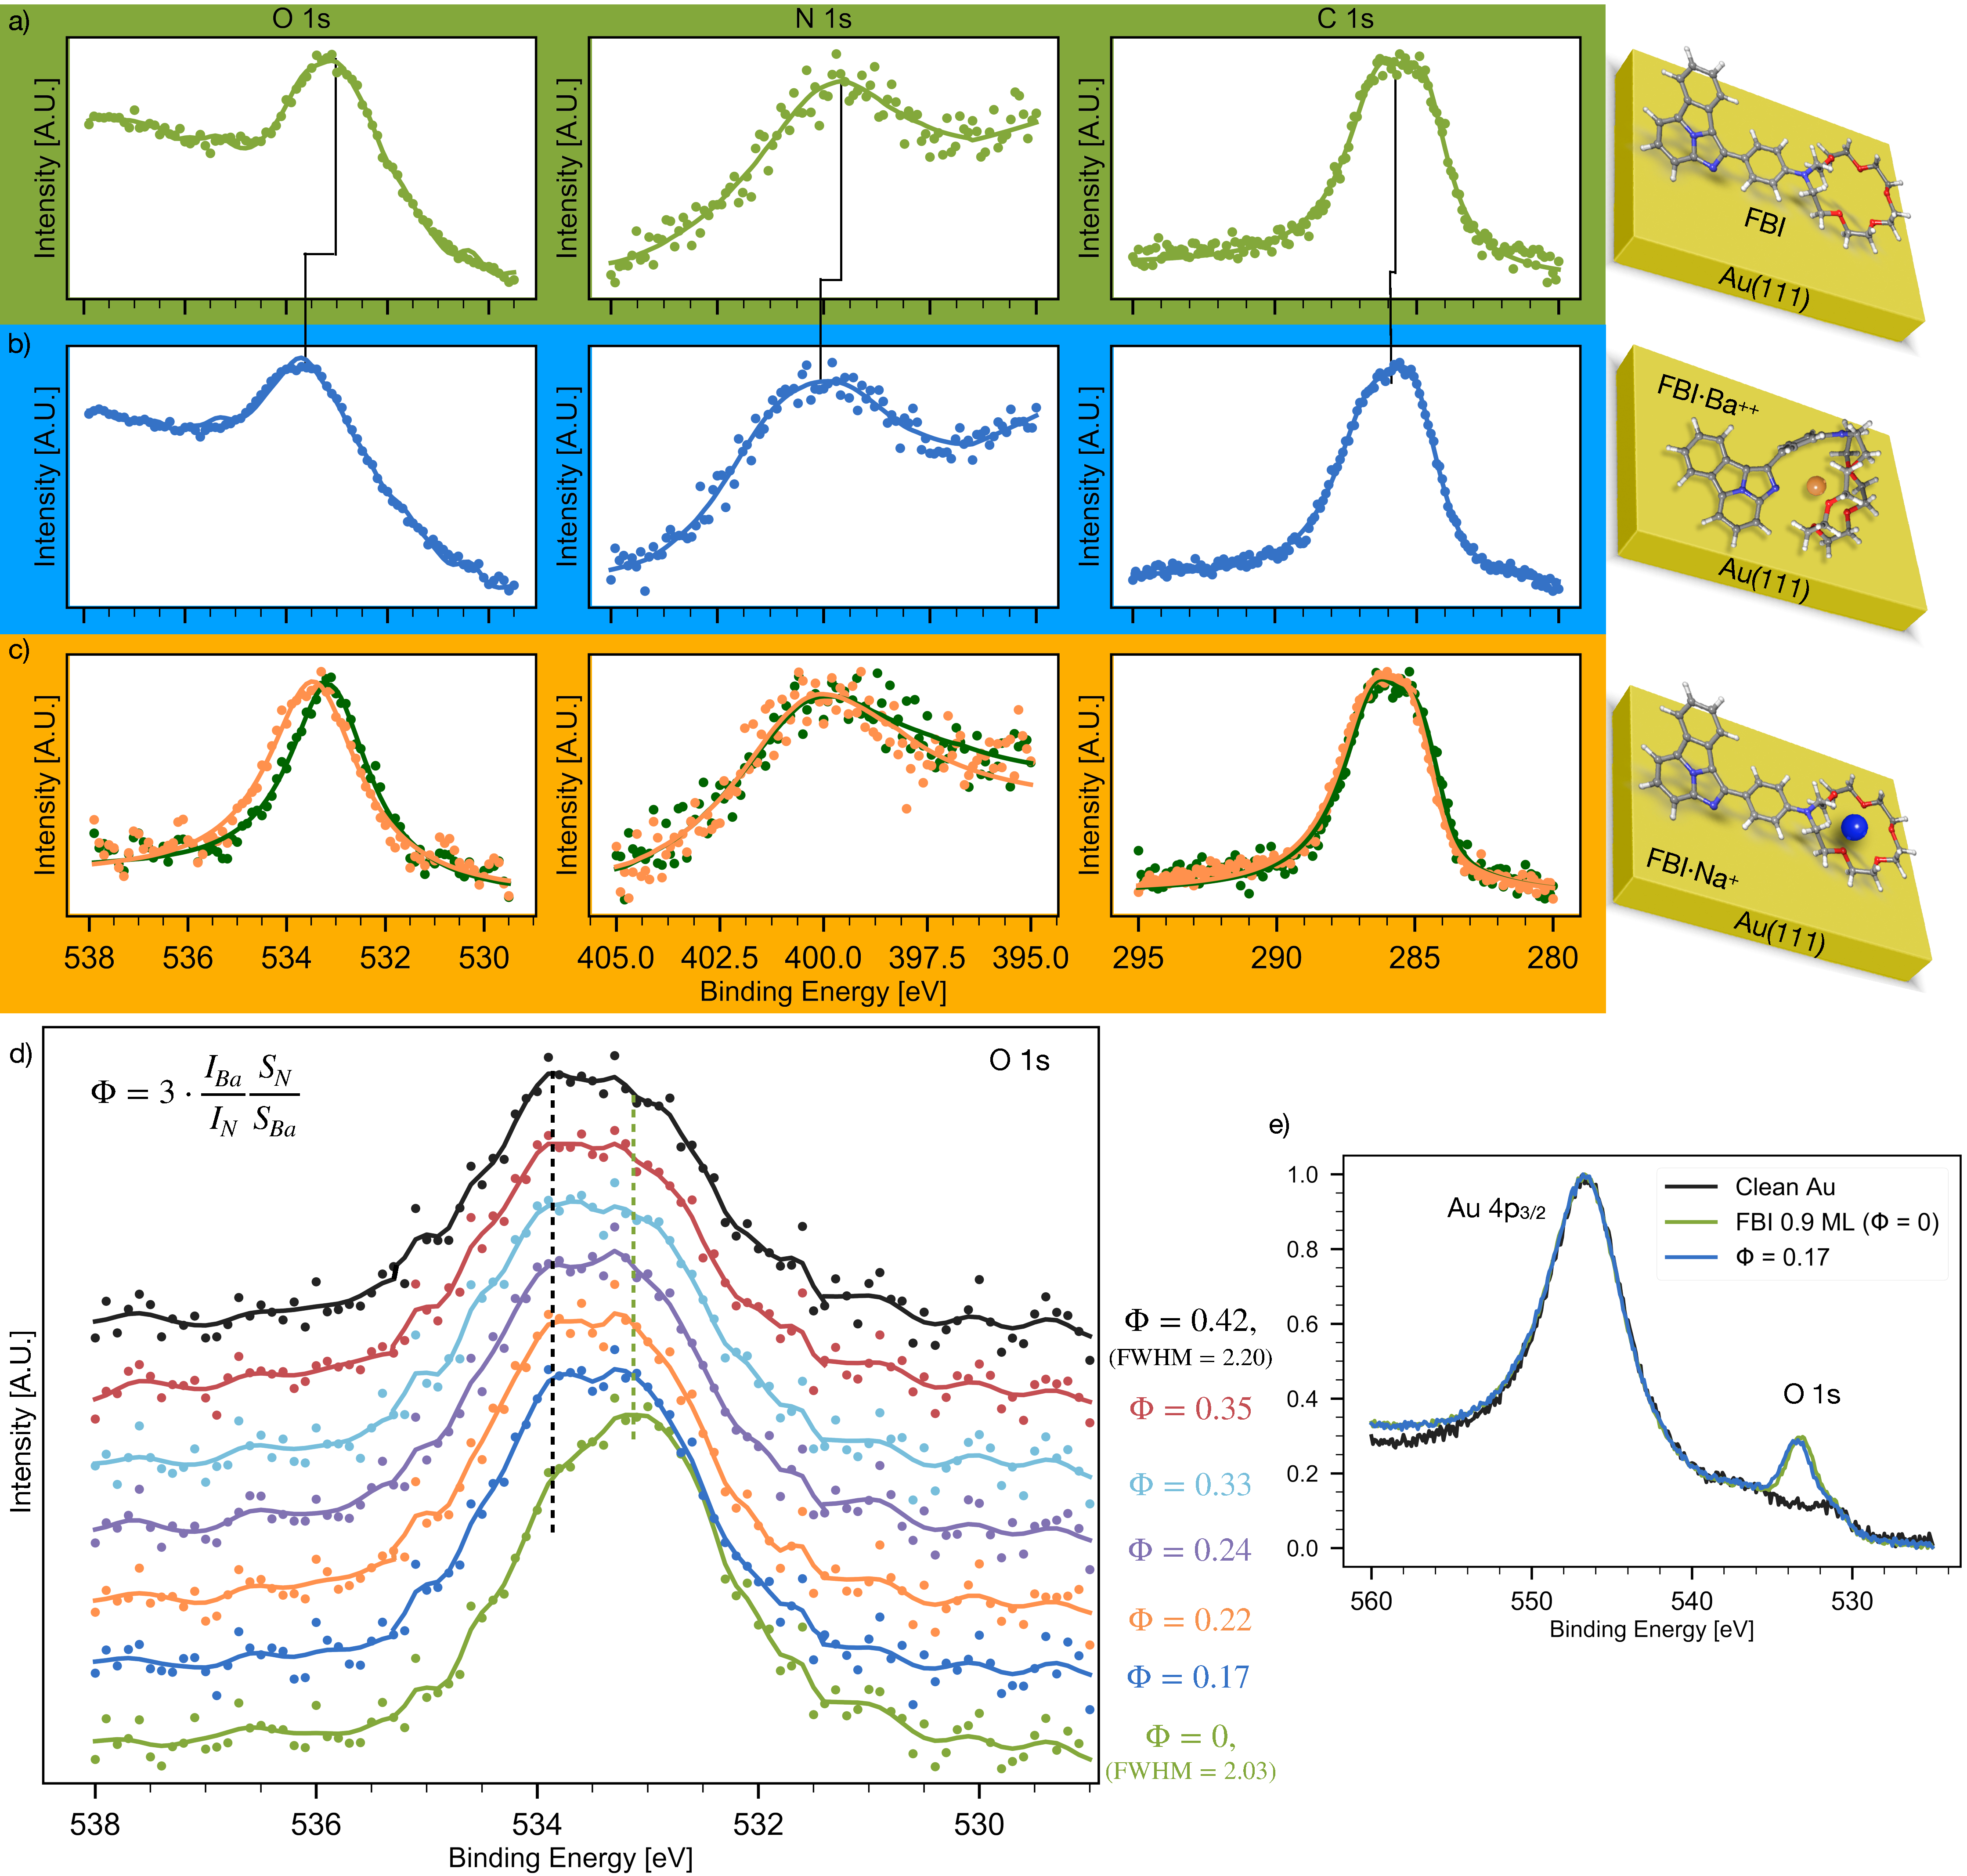
\includegraphics[width=0.99\textwidth]{figures/Fig2_a-d.pdf}
	\caption{\label{XPS_FBI_Au} 
    (a) XPS spectra on O 1s, N 1s and C 1s regions measured after 0.65 ML FBI deposition on Au(111); (b) after their chelation with 0.80 \Bapp per FBI molecule; (c) 2.60 \Nap per FBI molecule (orange line), and FBI previous to \Nap addition (green line). (d) Evolution of chelated component as a function of the \Bapp deposition.}
\end{figure*}  
\begin{figure*}[ht!]
	\includegraphics[width=0.9\textwidth]{figures/fig3_STM.pdf}
	\caption{\label{FIG_BRSTM} 
    (a) Large scale STM image of native FBI molecules upon deposition on Au(111) surface and measured at 4K. Red ovals show isolated molecules. Scale = 10 nm. Inserted Constant current STM image of an FBI molecule (I = 60 pA / U = 1.4 V) deposited on Au(111). (b) High resolution Bond-resolving STM image of the same FBI molecule with a CO-functionalized probe (constant height, U = 5 mV) (c) and (d) Bond-resolving STM image of sublimated FBI derivatives: only benzo[a]imidazo[5,1,2-cd]indolizine fluorophore (c) benzo[a]imidazo[5,1,2-cd]indolizine fluorophore with phenyl ring but without the crown ether (d).}
\end{figure*}

\section{Chemical demonstration of chelation}

For the chelation, \BappCl\ was sublimated on the FBI-functionalised Au(111) surface. When pure \BappCl\ was deposited on the Au(111) surface, its stoichiometry ratio Ba:Cl was 1:2 as expected. However, when it was deposited on {FBI-functionalised} Au(111), this ratio was around 1:1.3 and 1:1.6, meaning that some chlorine was desorbed when it reached the sample. From simulations \cite{rivilla_fluorescent_2020}, the {chloride ions are} expected to behave as {passive spectators} in the chelation, {which} is consistent {with their desorption} when the molecule is present.


After sublimation of 0.80 \Bapp per FBI molecule, the core levels, shown in figure {\bf \ref{XPS_FBI_Au}b}), are clearly shifted toward higher B.E, mainly on O 1s and N 1s. The maximum O 1s core level exhibits an upward chemical shift of 0.5 eV. This shift is not just a doping shift, but a real chemical change. This is revealed by the evolution of the O 1s for very low \Bapp doses on the surface. Figure {\bf \ref{XPS_FBI_Au}d} shows the evolution of the O 1s for incremental {amounts} of \Bapp ions. The Ba dose was {estimated} using the ratio between XPS intensities of spectra of Ba 2p and N 1s core level divided by the {corresponding} sensitivity factor, and always taking into account that there are 3 N atoms per molecule. Thus, the Ba per FBI molecule runs from 0 to almost 0.5 , i.e. until 2 FBI {molecules} per 1 \BappCl. The FBI coverage in this case is 0.9 ML. Once \BappCl\ is added to the sample, in the O 1s core level a second component, at higher binding energy appears, which makes that the peak width increases. At the latest stage of barium addition, the FWHM increases by 9\% with respect to the free state. We {deconvolved} the peaks after \Bapp addition using two components, one at 533.2 (FWHM = 2.20) corresponding to the free molecules and another at 533.8-534.0 eV, corresponding to chelated molecules. This is consistent with the molecules undergoing a chemical change upon chelation, as previously observed for crown ether chelation with Na \cite{stredansky_-surface_2019}.  The close proximity of the Au 4p core level affects the O 1s core level intensity (inserted for illustration in figure {\bf \ref{XPS_FBI_Au}d} hinder us to give an estimation of the chelation (trapping) efficiency. Mention that, in order to enhance the core level evolution and remark the spectral {series} shown in figure {\bf \ref{XPS_FBI_Au}d} corresponds to O 1s core region upon subtraction of the Au 4p contribution. 

To evaluate whether the nature of the dopant atom has any influence in the oxygen core level shift for the FBI molecules, we tested the chelation with \Nap. Thus, figure {\bf \ref{XPS_FBI_Au} c} shows the O 1s, N 1s and C 1s core levels measured on 0.6 ML of FBI on Au(111) before and after the sublimation of 2.60 \Nap per FBI. The maximum O 1s shift for \Nap-chelated FBI molecules is again 0.5 eV, excluding the nature of the ion as responsible of the shift. However no shift was detected for N 1s nor C 1s core levels. Having into account the high flexibility and mobility reported for the FBI molecules, this XPS discrepancy between \Bapp\- and \Nap-chelation can be interpreted as a first {proof} that {the molecular conformation of FBI and the cation-phenyl interaction vary} depending on the nature of the trapped ions. According to theoretical calculations, upon chelation with \Bapp, {FBI undergoes a structural torsion generated by the} interaction between {the ion, the iminic N atom of the benzo[\textit{a}]imidazo[5,1,2-\textit{cd}]indolizine moiety and the phenyl group of the unbound fluorophore} \cite{rivilla_fluorescent_2020}. On the contrary, in the case of \Nap the ion does not produce {this coordination pattern}  given its smaller size. 



\section{Molecular structural rearrangement induced by chelation}

In order to visualize the aforementioned structural changes undergone by the FBI molecules upon chelation along with the modified electronic properties as measured at the single molecule level, STM experiments were carried out. Thus, STM evidences of the findings are summarized in Figure \ref{Fig_STS}. 

\begin{figure*}[ht!]
	\includegraphics[width=0.9\textwidth]{figures/Fig_STS.png}
	\caption{\label{Fig_STS} 
    (a) Schematic diagram of metal intercalation. (b-d) STM images of (b) \Nap-complexed (U = 0.9 V, I = 60 pA), (c) native (U = 1.4 V, I = 60 pA), and (d) \Bapp-complexed (U = -1.8 V, I = 20 pA) FBI. (Scale bars = 0.5 nm) (e) STS spectra of native (dark), \Nap-complexed (red), and \Bapp-complexed (green) FBI.}
\end{figure*}


Figure \ref{Fig_STS}a shows the schematic representation of the FBI molecules before and after chelation with \Nap and \Bapp, whereas Fig. \ref{Fig_STS}b-d displays representative STM images next to each of the cases. The contrast in STM images is always determined by a convolution of topographical and electronic contributions. However, the observed changes in constant current mode images obtained at bias voltages well inside the molecular HOMO-LUMO gap still support the expected {conformational} changes. {In general,} complexation of crown ethers with alkali metals like \Nap causes the oxygen atoms to point to the center, forcing the ring to adopt a flatter conformation relative to the native molecule. Instead, calculations predict the FBI molecule to adopt a more three-dimensional conformation upon chelation with \Bapp. Taking into account that the three STM images are plotted with a common color code, it can be directly observed that the apparent heights of the crown ether follow the expected trend. Indeed, the apparent height for each of the molecules, as measured on the highest point of the crown, is 2.5$\pm$ 0.1 \AA, 2.1$\pm$ 0.1 \AA, and 2.9$\pm$ 0.1 \AA, for the pristine FBI and the \Nap and \Bapp chelated molecules, respectively.    
The associated STS spectroscopy revealed a HOMO-LUMO gap of 3.0 eV for the FBI molecule deposited on Au(111) (figure {\bf \ref{Fig_STS}e}). Complexation with \Nap did not considerably change this band gap, while complexation with \Bapp increased it to 3.6 eV. According to calculations, the HOMO and LUMO are mainly located around the dye and are determined by its $\pi$-network, with little contribution from the crown ether. A simple complexation between the crown ether and \Nap therefore does not change this gap substantially. This is in line with other dyes containing the same crown ether whose emission profiles do not change upon \Nap complexation.\cite{ast_high_2011} Meanwhile, the conformational change upon complexation with \Bapp causes a decrease in the extent of pi-conjugation, which no longer extends into the phenyl ring linking the fluorophore and the crown, consequently increasing the bandgap. This is in line with the changes in absorption and emission spectra. 

\begin{table}[]
    \centering
    \begin{tabular}{|c|c|c|c|c|}
        \hline
        Species &  Band gap / eV (nm) & $\lambda_{max}^{abs}$ / \text{nm} & $\lambda_{max}^{emi}$/\text{nm} \\ \hline
        FBI & 3.0 (413.3) & 432.5 & 485 \\
        FBI-\Nap & 3.1 (400.0) & 430 & 481 \\
        FBI-\Bapp & 3.6 (344.4) & 420.5 & 431 \\ \hline
    \end{tabular}
    \caption{Band gaps measured by STS on Au(111) vs absorption ($\lambda_{max}^{abs}$) \text{ and fluorescence emission} ($\lambda_{max}^{emi}$)\text{ spectral peaks.}}
    \label{tab:bandgaps}
\end{table}


%\begin{table}[]
%    \centering
%    \begin{tabular}{c|c|c|c|c}
%        Species &  Band gap [nm]  & Absorption peak [nm] & Emission peak [nm] \\
%        FBI-\Bapp & -68.9 & -12 & -32 \\
%        FBI-\Nap & -13.3 & ? & -3\\
%    \end{tabular}
%    \caption{Band gap, absorption and emission shifts with respect to unchelated FBI.}
%    \label{tab:wavelengthshifts}
%\end{table}

%\completar{Discuss about the molecular changes after chelation as well as relate the electronic changes with the changes in the fluorescence and relate this changes with the structural changes.} 


%\completar{If we include the calculation, then include a discussion about them.\textbf{ FER: OK, we can include the HOMO-LUMO gaps and the theoretical emission spectra for FBI and FBI·Ba(2+) to connect the structural changes (geometry) with the computational photophysics.}}


\section{Chelation independent of the surface support}

Finally we have also tested that chelation is taken place also in other surfaces, in particular Cu(111) and ITO. We chose Cu(111) because it is a more reactive substrate. This enabled us to study whether the molecule-substrate interaction could alter the chelation response. On the other hand, ITO was selected because it is a transparent substrate which allows the direct detection of fluorescence. Furthermore, the conductivity of ITO could enable guiding the \Bapp ions towards the surface in order for the molecules to capture it. These properties make ITO a promising candidate for the potential implementation of a barium tagging detector on a xenon-based TPC\cite{rivilla_fluorescent_2020}.

% For the Cu(111) sample, the Ba/FBI ratio = 10 (revised with proper area and ASF) i.e. much higher rate than for the Au(111) experiment. For the NaCl evaporation, the Na/FBI ratio = 3.66. 

% In the ITO sample, the Ba/FBI ratio = 17.5


As previously discussed the O 1s shift is a fingerprint of chelation. Figure \ref{XPS_FBI_Cu_ITO} shows the O 1s core level of FBI on Cu(111) and ITO. For Cu(111), we observed the same chemical shift on the O 1s (0.7 towards higher BE), indicating that chelation was also happening. In this case, the core level has a smaller component at lower B.E., around 531 eV, which is associated to residual contamination of the Cu surface in the form of Cu$_2$O \cite{zhu_surface_2013}.
The analysis of the shift for the case of ITO was not as direct because of the presence of oxygen in the ITO structure. To assess the differences associated to the FBI and chelated FBI molecules the core level measured on the ITO as prepared  was subtracted from that measured with FBI and BaCl$_2$. The result of the subtraction is shown in figure \ref{XPS_FBI_Cu_ITO} b), and the inset gathers the original normalized spectra, including the contribution from the ITO. From the 0.9 eV shift towards higher B.E. in figure \ref{XPS_FBI_Cu_ITO} b), we see that chelation is also taking place {on} ITO. These results ensure that chelation is independent from the choice of substrate, and that it is a property intrinsic to the molecule in conjugation with \Bapp. 


\begin{figure*}[ht!]
	\includegraphics[width=0.95\textwidth]{figures/fig5_cu_ito.pdf}
	\caption{\label{XPS_FBI_Cu_ITO} 
    a) O 1s core level spectra measured for FBI on Cu(111) and ITO surfaces before and after \Bapp sublimation. For ITO the substrate O 1s core level were substrates to emphasize the O 1s contribution coming from FBI.}
\end{figure*}  

\section{Conclusions}
This work establishes the suitability of the use of organic monolayer based devices as active component in a future neutrinoless double beta decay detector.

The demonstration of chelation in vacuum of FBI indicator by \Bapp\ ions once the molecules are deposited on suitable surfaces supports the barium tagging concept to achieve extremely low background xenon-based \bbonu\ {detection experiments}. Chemical and conformational changes that occur upon chelation, independently of the substrate where molecules were deposited, are in agreement with the calculations for the behaviour of free standing molecules, thus providing considerable freedom to choose the substrate. Moreover, the measured spectrum shifts are consistent with the observed {bicolour} property of the sensor for \Bapp\ ions compared to the {absence of} shift observed and predicted for other ions, such as \Nap.  
Furthermore, this study has also important implications beyond neutrino particle physics field. The capability of {aza-crown ethers} to interact with many different ions is very important in applications such as drug carriers \cite{uchegbu_non-ionic_1998} or photo-switching devices \cite{malval_photoswitching_2002,uda_membrane_2005}. 


\section{Methods}
The experiments were performed in two different UHV chambers, one for XPS experiments and the other for STM experiments. In both cases chambers has a base pressure of 1× 10-10 mbar. Prior to deposition, the Au(111) and Cu(111) and Indium Tin Oxide (ITO) surfaces was cleaned via cycles of Ar sputtering and annealing to 500°C and their cleanness was checked by XPS prior to molecular deposition. 

\textbf{Molecular evaporation}
Pure FBI, \BappCl and NaCl were evaporated from homemade Knudsen cell evaporators. To avoid cross talking between FBI and the salts molecules and to exclude any possibility of chelation of the molecule inside the cell, the FBI and \BappCl (NaCl) evaporators were located in two separated parts of the chambers. Same FBI, \BappCl and NaCl evaporators were used in both chambers (moved from one to the other) to ensure the reproducibility of sublimations.

FBI molecules were synthesis using the procedure described in REF.\cite{rivilla_fluorescent_2020} while \BappCl and NaCl were commercial (Sigma-Aldrich). The molecules were used after degassing in UHV.


\textbf{XPS experiments}
The XPS measurements were carried out using a SPECS Phoibos-100 electron analyzer, using a non monochromatic Al K$\alpha$ photon source, 1486.6 eV. The spectra were calibrated to the substrates main core level (Au 4f, Cu 2p, and In 3d, respectively). 
The evaporation thicknesses were estimated by XPS, studying the attenuation of the most intense substrate core level, i.e. Au 4f, Cu 2p and In 3d, respectivly. The calculations followed the guidelines provided in ref. \cite{powell_practical_2020}. We estimated the Electron Effective Attenuation (EAL) of electrons through the FBI layers for electrons with kinetic energies of 1402.6, 1041.6 and 554.61 eV (Au 4f 5/2, In 3d 5/2 and Cu 2p 3/2, respectively). The resulting EALs are 3.87, 3.05 and 1.85 nm, respectively. The thickness of the FBI samples was then estimated using the intensity of clean substrate core level as reference and the attenuated intensity after the evaporation. The amount of \Bapp (Na) per molecule were estimated by computing  the ratio $\theta=I_{Ba}/(I_N/3) \cdot S_N/S_{Ba} $, where $I_{Ba}$, $I_N$ is total area  of the  Ba 3d 5/2 and  N 1s  core  levels and $S_{Ba} = 25.84$, $S_N = 1.80$ are the corresponding atomic sensitivity factors\cite{scofield_hartree-slater_1976}. The factor 3 corresponds to considering 3 N atoms per molecule.

\textbf{STM experiments}
STM experiments were performed with a commercial Scienta-Omicron ultra-high vacuum LT-STM at 4.3 K. During the STM experiments, the tip was functionalized with CO (eventlually also with Cl) for high resolution STM (HR-STM) for the constant height dI/dV imaging. This was achieved by exposing the
sample to low pressure (approximately $1 \times 10^{-8}$ mbar) of CO whilst the sample was held below 7 K. CO molecules were then removed
from their adsorption sites via scanning over them or $\sim$ 2 V bias voltage pulses. Eventually tip was also functionalised with
Cl by vertically moving the tip close to the top of a NaCl island at a low bias voltage.

\bibliographystyle{apsrev4-1} 
\bibliography{literature_FBI}


%\section{Supplementary Information}
%\subsection{Data processing for O 1s on Au(111)}
%\begin{figure*}[ht!]
%	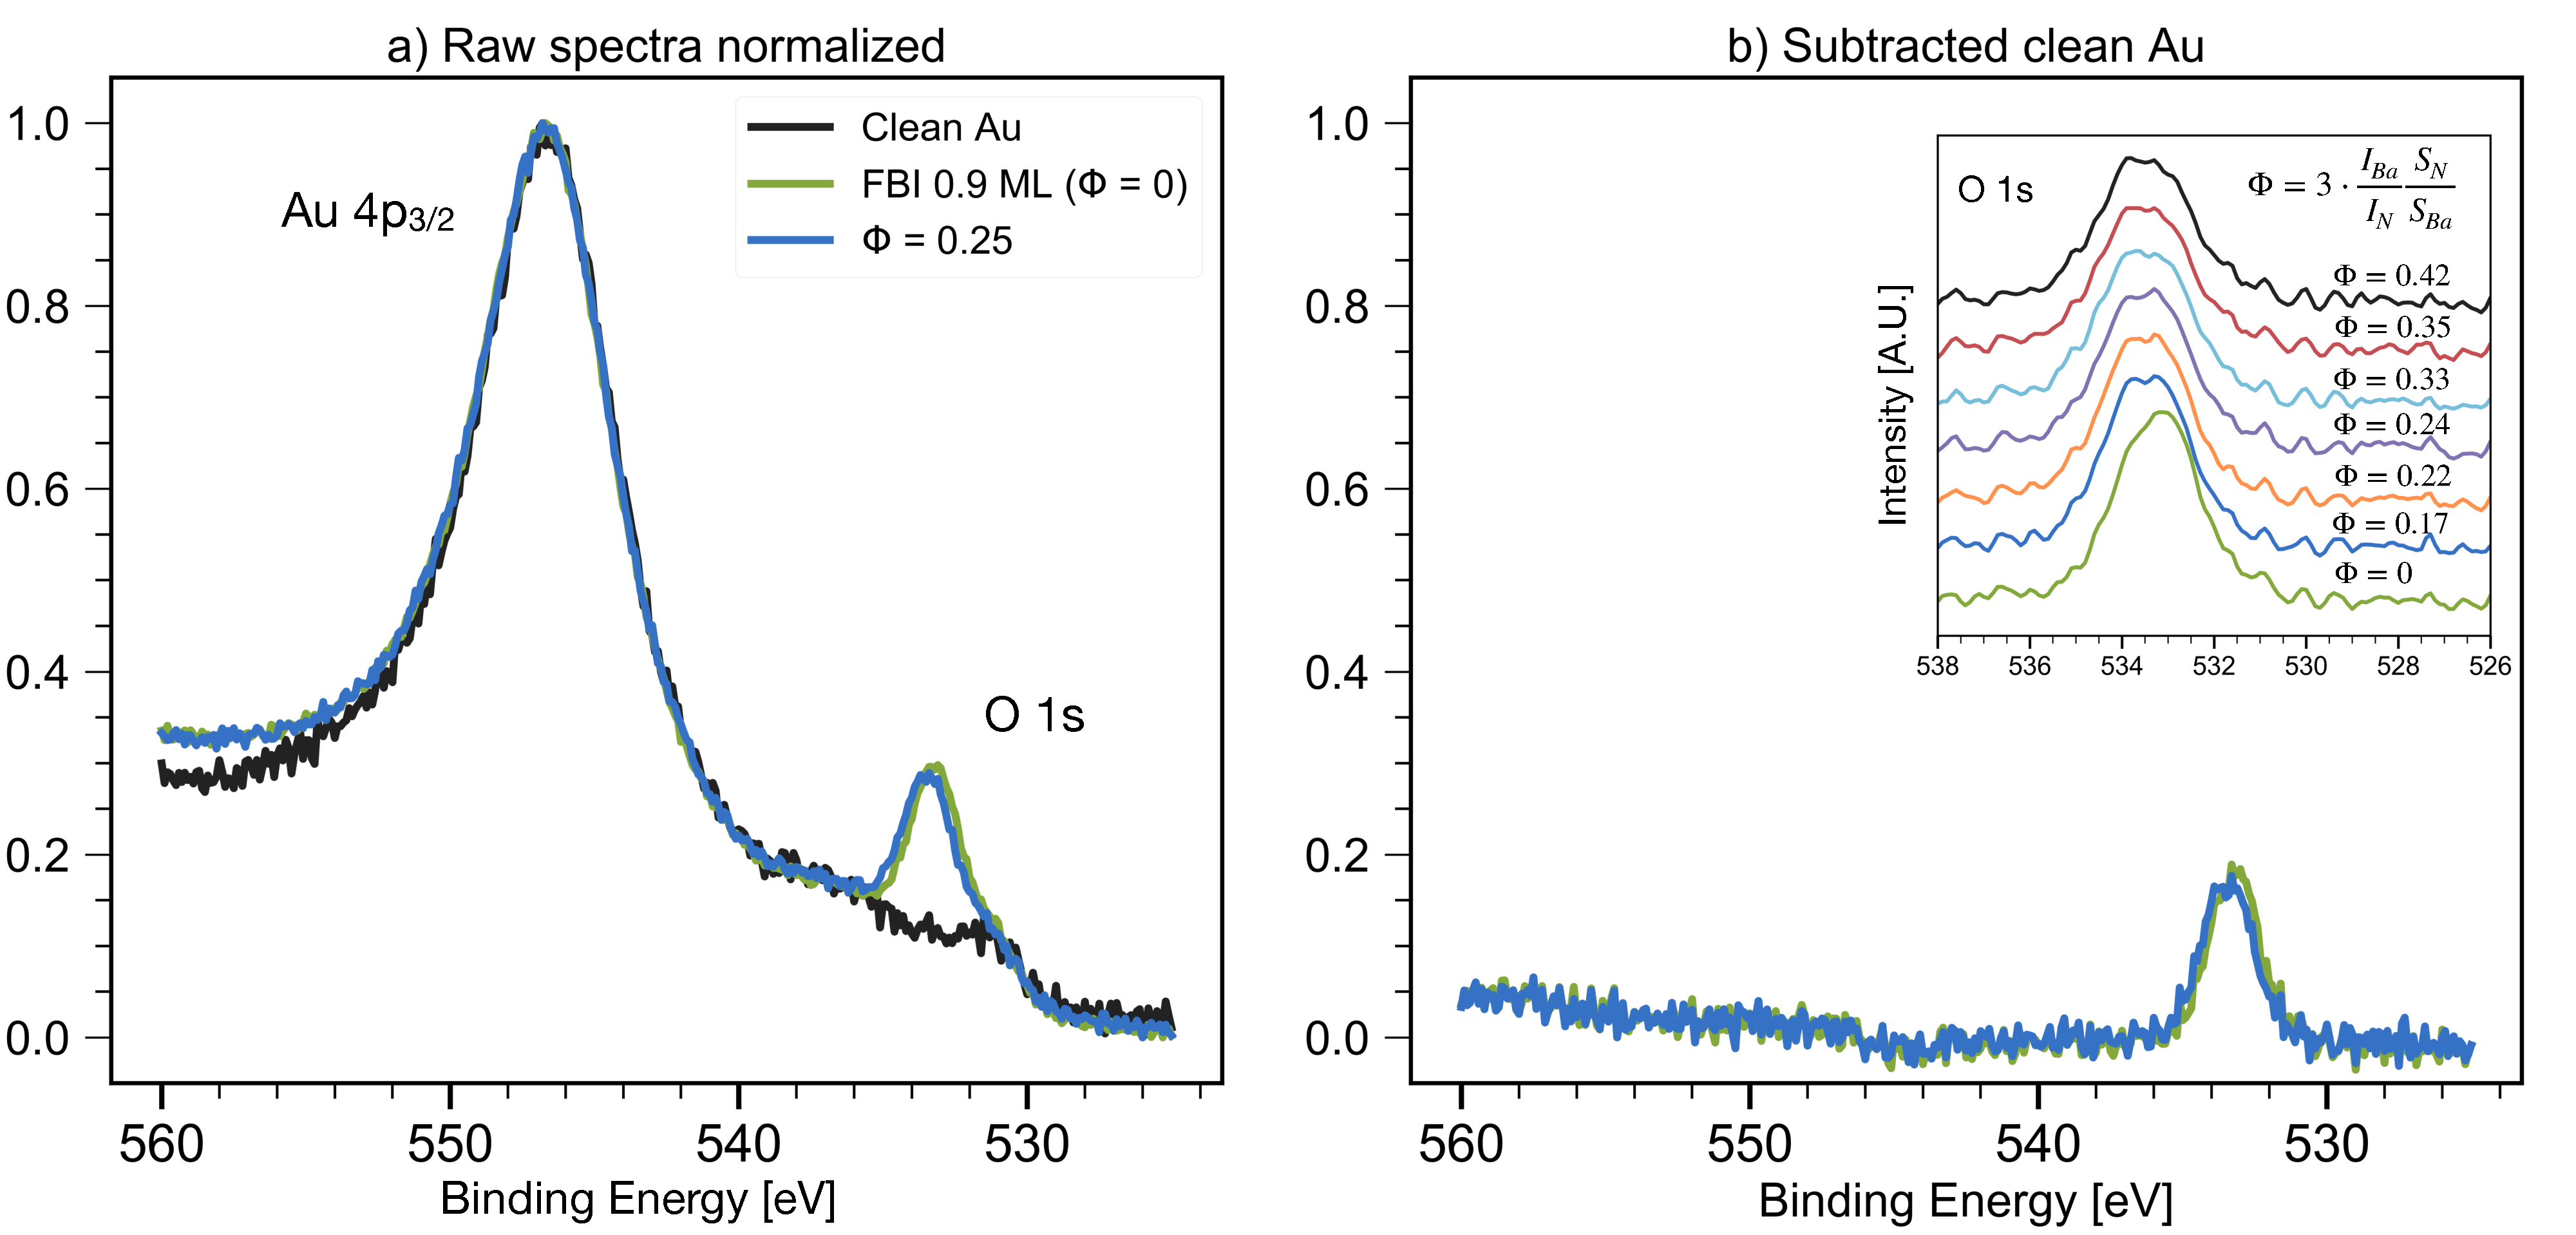
\includegraphics[width=0.9\textwidth]{figures/si_au_subtraction.pdf}
%	\caption{\label{Au_subtraction} 
%    XPS data treatment for O 1s core level in Au(111). The Au 4p core level contributes to the O 1s background. The intensity of the clean sample (red line) was subtracted from that corresponding to the deposition of FBI molecule (green line). To account for the attenuation of the Au 4p peak after evaporating the molecule, the maximum intensity of both curves was normalized to unity. The same treatment was applied to all lines in figure \ref{XPS_FBI_Au(111)} d) displayed here as inset.}
%\end{figure*}  

%%\subsection{Calculation of the Ba:Cl stoichiometry after sublimation}

%% This is outdated: the stoichiometry of pure BaCl2 was actually 2, as expected. We were computing wrong the area of the Ba 3d 5/2 peak. Also the Auger parameter was compatible with literature results for BaCl2

%%\begin{figure*}[ht!]
%	\includegraphics[width=0.9\textwidth]{figures/si_bacl_au_cu.png}
%	\caption{\label{Chlorine_desorption} \completar{Now } 
%    Evaporation of \BappCl directly (with no FBI molecule layer in between) on Cu(111) (black line) and Au(111) (red line). The stoichiometry ratio Cl/Ba, taking into account the atomic sensitivity factors (0.89 and 7.49 for Cl 2p and Ba 3d, respectively) is 0.7 and 0.64, for deposition in Au and Cu, respectively. Compare this to the expected ratio of 2 for the stoichiometric \BappCl salt. The intensity of chlorine did not change during the data acquisition, so desorption of chlorine due to the irradiation of X-rays was ruled out. Therefore, we attribute this low abundance of chlorine to the formation of gas Cl$_2$ either by interaction of the salt with the substrate or during the evaporation itself. In the case of NaCl evaporation, the presence of Cl 2p was below our detection sensitivity. The Ba 3d 5/2 and 3/2 peak are centered around 780.8 and 796.2 eV, respectively, which correspond to metallic barium \cite{jacobi_chemical_1987}. This is again consistent with the salt being dissociated and the barium stabilized upon interaction with the surface. Ba 3d from crystalline \BappCl would have these peaks centered around 777.5 and 792.8 eV (Ba 3d 5/2 and 3/2, respectively) \cite{kamada_solid-state_nodate}. Furthermore, the chemical state of barium in halides can be identified by differences in the ``Auger parameter" \cite{berrie_auger_1991, berrie_chemical_1994} $\alpha = KE(\mathrm{AES}) - KE(\mathrm{PE})$, i.e. the energy shift between a photoemission peak and the corresponding Auger peak. This parameter, when measured between the Ba 3d 5/2 and Ba M$_4$N$_{4,5}$N$_{4,5}$, takes values around 123.7 eV for BaO and \BappCl, whereas we measure a value of 105 eV. This value is compatible with that of metallic Ba \cite{vasquez_x-ray_1991}. The same holds for the state of barium in FBI-Ba samples: the Auger parameter is $\alpha = 109$ eV, and the Ba 3d 5/2, 3/2 peaks are centered around 780.9 and 796.2 eV, respectively.} 
%\end{figure*}  

%\begin{figure*}[ht!]
%	\includegraphics[width=0.9\textwidth]{figures/STMlarge.png}
%	\caption{\label{Large Scale STM images of FBI} 
 %   Large scale STM image of native FBI molecules upon deposition on Au(111). Red ovals show isolated molecules. Scale = 10 nm. }
%\end{figure*}  

\end{document}
